% multiple1902 <multiple1902@gmail.com>
% intro.tex
% Copyright 2011~2012, multiple1902 (Weisi Dai)
% https://code.google.com/p/xjtuthesis/
%
% It is strongly recommended that you read documentations located at
%   http://code.google.com/p/xjtuthesis/wiki/Landing?tm=6
% in advance of your compilation if you have not read them before.
%
% This work may be distributed and/or modified under the
% conditions of the LaTeX Project Public License, either version 1.3
% of this license or (at your option) any later version.
% The latest version of this license is in
%   http://www.latex-project.org/lppl.txt
% and version 1.3 or later is part of all distributions of LaTeX
% version 2005/12/01 or later.
%
% This work has the LPPL maintenance status `maintained'.
%
% The Current Maintainer of this work is Weisi Dai.
%

\chapter{基于法向量的缺陷检测算法}
\echapter{Normal Vector based Defect Detection Method}
由于基于基准面拟合的方法查准率较低,本章提出了基于法向量的缺陷检测算法,基于深度图像的法向量来检测缺陷区域,主要思路是利用法向量的余弦相似度来描述法向量的变化,根据输入的原始深度图像计算每个像素点的法向量,然后计算每个像素点与其邻域的法向量变化度量获得一张法向量梯度图像,接着根据法向量梯度图像使用双阈值分割获得候选的缺陷区域,最后验证候选区域的深度偏差是否达到了缺陷的定义,将满足缺陷定义的候选区域保留下来作为最终结果。
    \section{方法概述}
    \esection{Outline}
    钢板图像的缺陷区域往往在深度图像上表现为深度值上突然地落差,体现在法向量上能够理解为法向量的方向剧烈地变化。本算法根据法向量的余弦相似度来描述法向量之间的变化程度,对每一个像素点都计算其与邻域的法向量变化度量从而获得一张法向量梯度图像。法向量梯度图像直观的反映了深度值的平滑程度,法向量梯度值越大的地方越有可能是缺陷区域。

    该方法首先需要根据深度图像计算法向量,法向量一般被应用于点云数据的处理,深度图像本质上可以理解为结构化的点云数据。相对于在杂乱的点云上计算法向量,在深度图像上计算法向量要相对简单一些。Holzer等\cite{Holzer2012Adaptive}提出了两种利用积分图在深度图像上计算法向量的方法,第一种是根据水平向量和垂直向量的叉积来计算法向量,第二种是利用协方差矩阵来计算法向量。第一种法向量计算方法根据图像深度的变换求出对应点的水平向量和垂直向量,然后求出水平向量和垂直向量的叉积就得到法向量。第二种法向量计算方法利用协方差矩阵来计算法向量,根据对应点的领域信息,先计算它们的相应的协方差矩阵,然后计算这个协方差矩阵的特征向量,对应于最小特征值的特征向量就是计算得到的法向量,相较于利用叉积求法向量的方法,该方法虽然更加复杂和费时,但是利用协方差矩阵求法向量的方法更加准确可靠,并且协方差的特征向量能够直接体现对应点的领域平面的平面特性。我们主要使用基于协方差矩阵的方法来计算法向量,这种方法计算出的法向量更为平滑可靠。计算得到每个像素点的法向量之后,根据余弦相似度来计算法向量梯度图像,法向量梯度图像概念上类似于灰度图像的梯度图,主要用来检测法向量的变化情况。接着,使用双阈值分割来对法向量梯度图像进行二值化获得缺陷候选区域,最后对每个缺陷候选区域进行深度验证,检测其深度偏差是否达到缺陷的定义,最后把满足缺陷的深度定义条件的缺陷候选项输出作为最终的结果。

    基于法向量的缺陷检测算法流程如图\ref{fig:c5_flow_chart}所示,包括了计算法向量梯度图像,双阈值分割以及深度验证。

    \begin{figure*}[!h]
    \centering
    
\includegraphics[width=16cm]{c5_flow_chart.png}
    \caption{基于法向量的缺陷检测算法流程图}
    \label{fig:c5_flow_chart}
    \end{figure*}

    \section{计算法向量梯度图}
    \esection{Gradient Map of Normal Vector}
    法向量是指垂直于某一个平面的向量,对于一副深度图像而言,每个像素点跟其邻域的像素点能够拟合出一个局部的平面,该平面的法向量就是这个像素点的法向量,法向量的方向能够很好的表示出深度图像上的深度变化。

    法向量一般被应用于点云数据的处理,深度图像本质上可以理解为结构化的点云数据。相对于在杂乱的点云上计算法向量,在深度图像上计算法向量要相对简单一些。Holzer等\cite{Holzer2012Adaptive}提出了两种利用积分图来计算法向量的方法,第一种是根据水平向量和垂直向量的叉积来计算法向量,第二种是利用协方差矩阵来计算法向量。我们主要使用基于协方差矩阵的方法来计算法向量,这种方法计算出的法向量更为平滑可靠。

    在文章\cite{Holzer2012Adaptive}中,作者提出了两种法向量计算方法,并且采用了自适应的策略来确定计算法向量时领域半径的参数。第一种法向量计算方法根据图像深度的变换求出对应点的水平向量和垂直向量,然后求出水平向量和垂直向量的叉积就得到法向量。其原理如图\ref{fig:c5_normal_vector}所示。

    \begin{figure*}[!h]
    \centering
    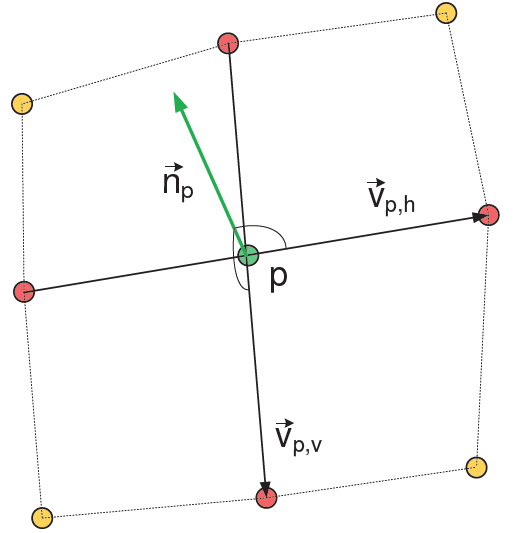
\includegraphics[width=8cm]{c5_normal_vector.png}
    \caption{法向量计算原理}
    \label{fig:c5_normal_vector}
    \end{figure*}

    第二种法向量计算方法利用协方差矩阵来计算法向量,根据对应点的领域信息,先计算它们的相应的协方差矩阵,然后计算这个协方差矩阵的特征向量,对应于最小特征值的特征向量就是计算得到的法向量,相较于利用叉积求法向量的方法,该方法虽然更加复杂和费时,但是利用协方差矩阵求法向量的方法更加准确可靠,并且协方差的特征向量能够直接体现对应点的领域平面的平面特性。

    计算得到每个像素点的法向量之后,根据余弦相似度来计算法向量梯度图像,法向量梯度图像概念上类似于灰度图像的梯度图,主要用来检测法向量的变化情况。假定$N\left({r,c}\right)$代表了点$\left({r,c}\right)$的法向量,那么点$\left({r,c}\right)$的法向量梯度值$g_n\left({r,c}\right)$表示为:
    \begin{eqnarray}
    g_n\left({r,c}\right)=\sqrt{{g_h\left({r,c}\right)}^{2}+{g_v\left({r,c}\right)}^{2}}
    \end{eqnarray}
    其中$g_h\left({r,c}\right)$和$g_v\left({r,c}\right)$分别表示为点$\left({r,c}\right)$ 在水平方向和垂直方向上的梯度值。$g_h\left({r,c}\right)$和$g_v\left({r,c}\right)$的公式表达为:
    \begin{eqnarray}
    g_h\left({r,c}\right)=C\left({N\left({r,c}\right),N\left({r,c-1}\right)}\right)+C\left({N\left({r,c}\right),N\left({r,c+1}\right)}\right)
    \end{eqnarray}
    \begin{eqnarray}
    g_v\left({r,c}\right)=C\left({N\left({r,c}\right),N\left({r-1,c}\right)}\right)+C\left({N\left({r,c}\right),N\left({r+1,c}\right)}\right)
    \end{eqnarray}
    公式中函数$C$表示计算计算两个法向量之间的相似性度量,函数$C$的公式为:
    \begin{eqnarray}
    C\left({n_1,n_2}\right)=1-abs\left({\frac{dot\left({n_1,n_2}\right)}{{\left\|n_1\right\|}_2*{\left\|n_2\right\|}_2}}\right)
    \end{eqnarray}
    其中$abs$函数为求绝对值函数,$dot$函数表示求两个向量的点积,${\left\|n\right\|}_2$ 定义为向量$n$的二范数。

    在扫描完整张图像,对每个像素点都计算得到其法向量梯度值之后,我们就得到了一张法向量梯度图像。法向量梯度图像非常类似于灰度图像的梯度图,不同的是法向量梯度图像表示一个邻域内法向量方向的变化,而灰度图像的梯度图表示灰度值的变化。

    法向量梯度图像的效果如图\ref{fig:c5_gradient}所示,从左至右依次为深度图像三维伪彩图、法向量梯度图像。

    \begin{figure*}[!h]
    \centering
    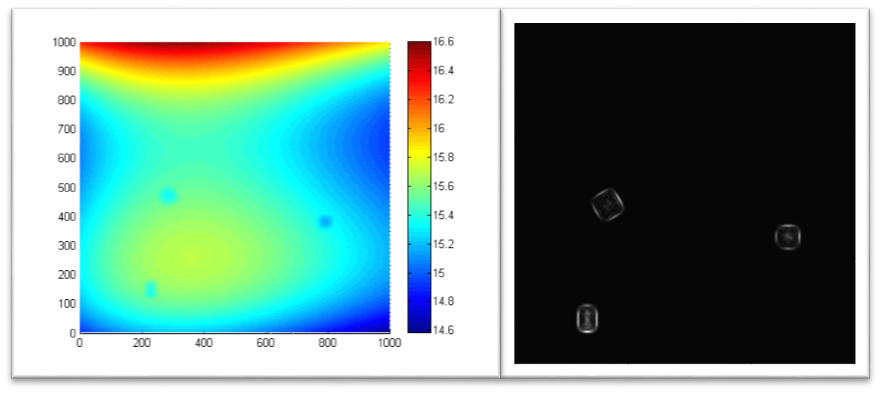
\includegraphics[width=16cm]{c5_gradient.png}
    \caption{法向量梯度图像}
    \label{fig:c5_gradient}
    \end{figure*}

    \section{双阈值分割}
    \esection{Dual Threshold Segmentation}
    在钢板缺陷检测领域,双阈值分割使用地非常频繁,这种类似于canny边缘算子\cite{Canny1986A} 的高低阈值设置方式在工程上被认为是简单可行并切实有效的。

    对法向量梯度图像使用高低阈值分别分割之后,获得了两张二值图像。双阈值分割的公式一般表达为:
    \begin{eqnarray}
    \left\{ \begin{array}{l}
    {B_{high}}\left( {r,c} \right) = 1,{g_n}\left( {r,c} \right) > {T_{high}}\\
    {B_{high}}\left( {r,c} \right) = 0,otherwise
    \end{array} \right.
    \end{eqnarray}
    \begin{eqnarray}
    \left\{ \begin{array}{l}
    {B_{low}}\left( {r,c} \right) = 1,{g_n}\left( {r,c} \right) > {T_{low}}\\
    {B_{low}}\left( {r,c} \right) = 0,otherwise
    \end{array} \right.
    \end{eqnarray}
    分割后的二值图像描述了缺陷区域的边缘信息,然而我们更关心的是缺陷部分的连通区域。所以我们首先使用3x3的正方形形态学算子对低阈值二值图像进行膨胀操作将一些断裂的边缘重新连接起来,接着对膨胀后的二值图像使用孔洞填充算法填充边缘二值图像的内部区域。接着对二值图像使用二值标记算法来获取候选缺陷连通区域获得两张连通区域标记图像${L_{low}}\left( n \right)$和${L_{high}}\left( m \right)$($n$和$m$表示连通区域的标记索引,$n = 1, \ldots ,N$,$m = 1, \ldots ,M$)。对低阈值连通区域标记图像$L_{low}$中的任一连通区域,如果它包含了高阈值连通区域标记图像$L_{high}$的连通区域,就将它保留,否则,舍弃。这个过程公式为:
    \begin{eqnarray}
    \left\{ \begin{array}{l}
    {B_{double}}\left( {{L_{low}}\left( n \right)} \right) = 1,{L_{high}}\left( m \right) \subset {L_{low}}\left( n \right)\\
    {B_{double}}\left( {{L_{low}}\left( n \right)} \right) = 0,otherwise
    \end{array} \right.
    \end{eqnarray}
    假定$L\left(i\right)$表示连通区域标记图像$L$中索引为$i$的连通区域的点集。经过双阈值分割后,最终分割出来的二值图像$B_{double}$中的连通区域就是候选的缺陷区域。在双阈值分割过程中,高低阈值$T_{high}$和$T_{low}$的选择比较重要,高阈值$T_{high}$的设置需要使得分割出来的二值图像查准率尽可能高,而低阈值$T_{low}$的设置需要使得查全率尽可能高。

    双阈值分割的结果如图\ref{fig:c5_double_thresh}所示,从左至右依次为法向量梯度图像、高阈值分割二值图、低阈值分割二值图、最终结果。

    \begin{figure*}[!h]
    \centering
    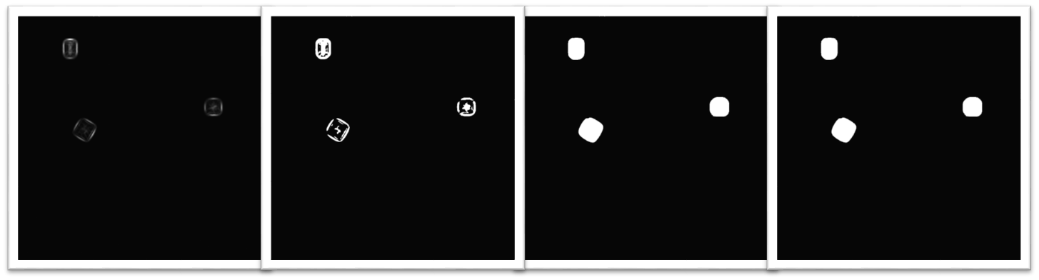
\includegraphics[width=16cm]{c5_double_thresh.png}
    \caption{双阈值分割实验结果}
    \label{fig:c5_double_thresh}
    \end{figure*}

    \section{深度验证}
    \esection{Verification of Depth}
    法向量梯度图像表示了像素点法向量变化的显著程度,所以在法向量梯度图像上分割后获得的连通区域在其边缘上法向量改变较明显。这一特点符合缺陷的特征,然而并不充分,因为根据定义缺陷不仅在其边缘上法向量存在剧烈的变化,其深度相对于正常钢板平面也存在较大的差异,所以对于每个候选的缺陷区域,都需要进行深度值的验证。

    对于一个候选的缺陷区域,首先对其矩形包围盒进行扩大,保持矩形包围盒的中心不变,将其长宽都扩大为之前的3倍,这样做是为了获得候选缺陷区域周边的局部上下文信息。接着对扩大后的局部深度图像使用章节4.2中的基准面拟合方法拟合出基准面,然后根据局部深度图像和基准面计算连通区域内每个像素点的深度偏差的最大值,若该最大值大于某个阈值,则保留该连通区域作为缺陷区域。这一过程用公式表达为:
    \begin{eqnarray}
    \left\{ \begin{array}{l}
    Label\left( i \right) = 1,\mathop {\max }\limits_{k \in P\left( i \right)} \left( {{d_{norm}}\left( k \right) - f\left( k \right)} \right) > {T_{depth}}\\
    Label\left( i \right) = 0,otherwise
    \end{array} \right.
    \end{eqnarray}
    其中$label\left(i\right)$表示对索引为$i$的连通区域的标记,其值为1代表作为缺陷保留,为0代表舍弃,$P\left(i\right)$代表该连通区域的点集。$k$代表一个像素点,$d_{norm}\left(k\right)$和$f\left(k\right)$分别代表该像素点在基准面的深度值和原始深度图像的深度值。

    \section{实验结果}
    \esection{Experimental Results}
        \subsection{数据集与评价方法}
        \esubsection{Data-set and Evaluation Protocol}
        本章的方法使用章节4.5.1提出的人工合成钢板深度图像数据集来检测算法的效果。同样的,对于检测算法检出的一个缺陷连通区域,我们使用连通区域包围盒的重叠率来判断检测是否成功,假定$R_p$为检测算法检测出的缺陷连通区域包围盒,$R_t$是已标记的缺陷连通区域包围盒,若$\frac{{R_p}\bigcap{R_t}}{{R_p}\bigcup{R_t}}>T_{overlap}$,即包围盒重叠率大于某个阈值则认为检测算法检出的该连通区域是一个缺陷。我们使用查全率、查准率和F值来评价算法的最终检测效果。
        \subsection{实验结果与分析}
        \esubsection{Experimental Results and Analysis}
        我们使用Matlab语言实现了本文提出的两个深度图像缺陷检测算法,实验用的计算机配置为:Intel Xeon E3-1241 3.50GHz CPU、32GB内存、Windows 7操作系统。处理一张1000x1000的深度图像,基于法向量的方法平均处理时间为60s。

        基于协方差矩阵来计算法向量,根据对应点的领域信息,先计算它们的相应的协方差矩阵,然后计算这个协方差矩阵的特征向量,对应于最小特征值的特征向量就是计算得到的法向量。使用MATLAB实现的部分代码如下所示,这部分代码实现了利用协方差矩阵来求解法向量。

        \lstinputlisting{code/get_normal_vector2.m}

        计算得到每个像素点的法向量之后,根据余弦相似度来计算法向量的梯度图像,法向量梯度图像在概念上类似于灰度图像的梯度图,主要用来检测法向量的变化情况。下面这部分代码实现了根据每个点的法向量来计算法向量梯度图像。

        \lstinputlisting{code/get_gradient_from_normal_vector.m}

        基于法向量的方法利用了缺陷部分的法向量变化较为剧烈这一特征,使用法向量梯度图像来刻画法向量的变化程度,概念上类似于灰度图像的梯度图,接着使用双阈值分割来获得候选缺陷区域,最终使用深度验证来确定候选缺陷区域是否为真正的缺陷。下面这部分代码表示了基于法向量方法检测缺陷的基本流程。

        \lstinputlisting{code/normal_detect_defect.m}

        本章中提出的基于法向量的深度图像缺陷检测算法在人工合成深度图像数据集上进行了实验,并评估了实验结果,实验结果如表\ref{tbl:c5_nvector_result}所示:

        \begin{table*}[!h]
        \centering
        \caption{基于法向量方法的实验结果}
        \label{tbl:c5_nvector_result}
        \begin{tabularx}{\columnwidth}{>{\centering\arraybackslash}X >{\centering\arraybackslash}X >{\centering\arraybackslash}X >{\centering\arraybackslash}X}
        \toprule
        方法 & 查全率 & 查准率 & F值 \\
        \midrule
        基于法向量 & 0.872 & 0.99 & 0.927 \\
        \bottomrule
        \end{tabularx}
        \end{table*}

        对于基于法向量的方法,输入可以是结构化点云数据,也可以是深度图像。由于深度图像只给出的每个像素点世界坐标系下的z轴坐标,没有x坐标和y坐标的信息,所以我们使用深度图像的像素坐标系的x坐标和y坐标来代替世界坐标系下的x坐标和y坐标。因为像素坐标系与世界坐标系之间可以通过单应性矩阵相互转换,这样做实际上并不会影响最终的实验效果,但是双阈值分割时阈值的设定会不一样。我们在实验中输入深度图像,使用协方差矩阵方法计算法向量时窗口半径设置为5,双阈值分割时高阈值$T_{high}$设置为$1*{10}^{-6}$,低阈值$T_{low}$ 设置为$T_{high}*0.1$,跟基于基准面的缺陷检测算法相同,深度验证时$T_{depth}$设置为0.1mm。

        本章提出的基于法向量的深度图像缺陷检测算法在人工合成的数据集上都达到了令人满意的效果。基于法向量的方法查准率较高,误检的情况较少,但是其查全率较低,存在缺陷未能检出的情况,主要原因可能是双阈值分割时阈值的设定较为苛刻。

        相比较与基于基准面拟合的缺陷检测算法,基于法向量的缺陷检测算法查准率较高,但是查全率相对较低,分析实验结果,基于法向量的缺陷检测算法容易漏检一些较小的缺陷,主要是因为较小的缺陷其法向量的变化程度相对不明显,所以反应在法向量的梯度图像上其梯度值较低,另外基于法向量的缺陷检测算法中,由于我们采用的是固定阈值,双阈值分割的高低阈值选择都需要足够的实验来确定,若想要提高查全率,可以尝试降低分割阈值,而这样做可能导致误检,降低查准率,所以基于法向量的方法阈值的确定较为困难。

        基于基准面拟合的方法往往能够分割出完整的缺陷轮廓,因为其最后一步采用了SFM水平集图像分割算法,而基于法向量的方法,由于其采用了形态学操作对分割后的二值图像进行了处理来将可能断裂的缺陷区域连接起来,其最终检出的缺陷轮廓并不完全准确,在实际应用中,缺陷轮廓并不准确影响并不大,钢厂一般更关心缺陷是否成功检出以及缺陷的位置,然而在实验评价中,基于法向量的方法处于劣势,可能有些缺陷区域基于法向量的方法实际上已经检出,但是由于检出的连通区域相对于groundtruth过大或者过小,导致被评价方法认定为没有检出。

        在人工合成数据集上的部分实验结果如图\ref{fig:c5_nvector_result}所示,从左至右依次为深度图像三维伪彩图、标记的缺陷区域、基于法向量算法的检测结果。

        \begin{figure*}[!h]
        \centering
        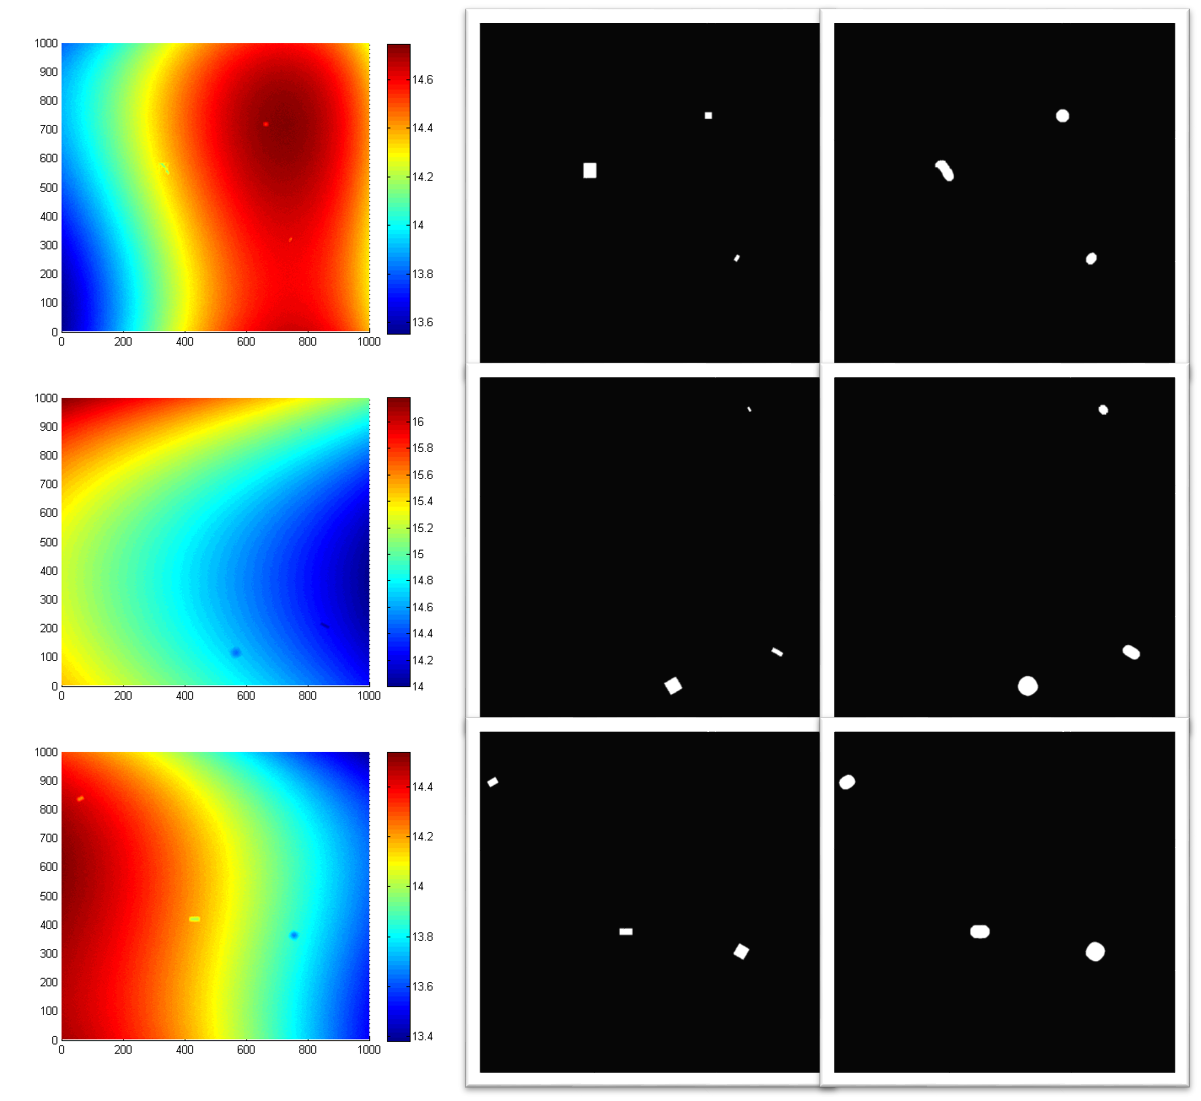
\includegraphics[width=16cm]{c5_nvector_result.png}
        \caption{基于法向量方法的部分实验结果}
        \label{fig:c5_nvector_result}
        \end{figure*}

    \section{本章小结}
    \esection{Brief Summary}
    在本章中,我们提出了一种基于法向量的深度图像缺陷检测算法。基于法向量的方法利用了缺陷部分的法向量变化较为剧烈这一特征,使用法向量梯度图像来刻画法向量的变化程度,概念上类似于灰度图像的梯度图,接着使用双阈值分割来获得候选缺陷区域,最终使用深度验证来确定候选缺陷区域是否为真正的缺陷。

